\documentclass[11pt,fleqn]{article}
\usepackage{../cs188,latexsym,epsf, amsmath,amsfonts,graphicx,url,multicol}
\usepackage{caption}
\usepackage{subcaption}
\lecture{5}
\def\title{Note \the\lecturenumber}
\begin{document}
\maketitle


\iffalse
\documentclass[11pt,fleqn]{article}
\usepackage{latexsym,epsf,amsmath,amsfonts,graphicx,url}

\title{Note 5}

\newcommand{\F}{\mathbb{F}}
\newcommand{\Z}{\mathbb{Z}}
\newcommand{\Q}{\mathbb{Q}}
\newcommand{\R}{\mathbb{R}}
\newcommand{\C}{\mathbb{C}}

\begin{document}

\maketitle
\fi

\section*{Reinforcement Learning}
In the previous note, we discussed Markov decision processes, which we solved using techniques such as value iteration and policy iteration to compute the optimal values of states and extract optimal policies. Solving Markov decision processes is an example of \textbf{offline planning}, where agents have full knowledge of both the transition function and the reward function, all the information they need to precompute optimal actions in the world encoded by the MDP without ever actually taking any actions. In this note, we'll discuss \textbf{online planning}, during which an agent has no prior knowledge of rewards or transitions in the world (still represented as a MDP). In online planning, an agent must try \textbf{exploration}, during which it performs actions and receives \textbf{feedback} in the form of the successor states it arrives in and the corresponding rewards it reaps. The agent uses this feedback to estimate an optimal policy through a process known as \textbf{reinforcement learning} before using this estimated policy for \textbf{exploitation}, or reward maximization.
\begin{center}	
	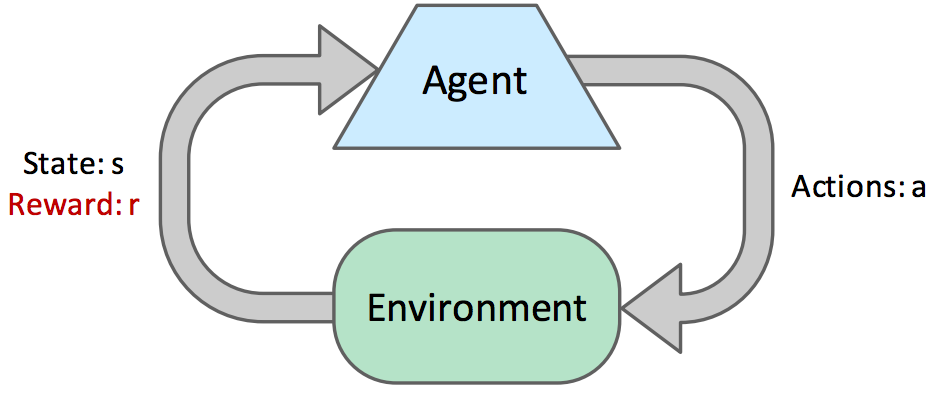
\includegraphics[width=10cm]{img/feedback-loop}
\end{center}
Let's start with some basic terminology. At each timestep during online planning, an agent starts in a state $s$, then takes an action $a$ and ends up in a successor state $s'$, attaining some reward $r$. Each $(s, a, s', r)$ tuple is known as a \textbf{sample}. Often, an agent continues to take actions and collect samples in succession until arriving at a terminal state. Such a string of samples is known as an \textbf{episode}. Agents typically go through many episodes during exploration in order to collect sufficient data needed for learning.

There are two types of reinforcement learning, \textbf{model-based learning} and \textbf{model-free learning}. Model-based learning attempts to estimate the transition and reward functions with the samples attained during exploration before using these estimates to solve the MDP normally with value or policy iteration. Model-free learning, on the other hand, attempts to estimate the q-values of states directly, without ever using any memory to construct a model of the rewards and transitions in the MDP. 

\section*{Model-Based Learning}
In model-based learning an agent generates an approximation of the transition function, $\hat{T}(s, a, s')$, by keeping counts of the number of times it arrives in each state $s'$ after entering each q-state $(s, a)$. The agent can then generate the the approximate transition function $\hat{T}$ upon request by \textbf{normalizing} the counts it has collected - dividing the count for each observed tuple $(s, a, s')$ by the sum over the counts for all instances where the agent was in q-state $(s, a)$. Normalization of counts scales them such that they sum to one, allowing them to be interpreted as probabilities. Consider the following example MDP with states $S = \{A, B, C, D, E, x\}$, with $x$ representing the terminal state, and discount factor $\gamma = 1$:
	\begin{center}
		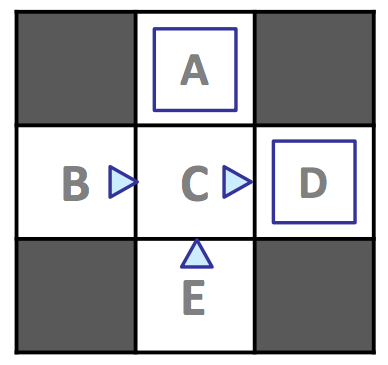
\includegraphics[width=5cm]{img/rl-example-1}
	\end{center}
Assume we allow our agent to explore the MDP for four episodes under the policy $\pi_{explore}$ delineated above (a directional triangle indicates motion in the direction the triangle points, and a blue squares represents taking $exit$ as the action of choice), and yield the following results:
	\begin{center}
		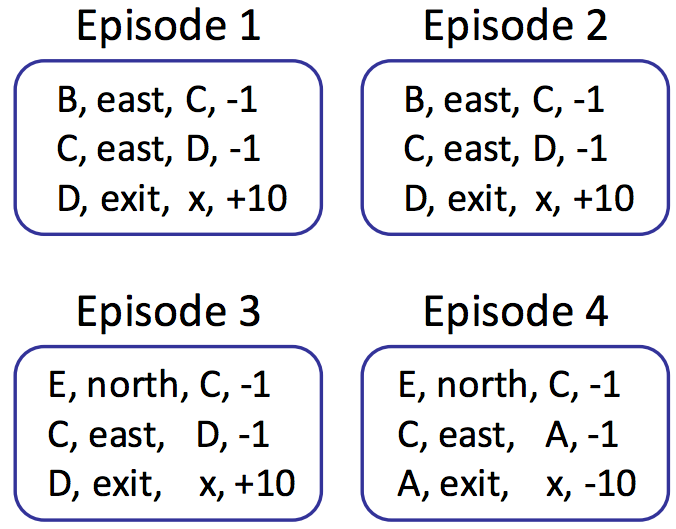
\includegraphics[width=8cm]{img/example-1-episodes}
	\end{center}
We now have a collective $12$ samples, $3$ from each episode with counts as follows:
\begin{center}
\begin{tabular}{ |c|c|c|c| } 
 \hline
 \textbf{s} & \textbf{a} & \textbf{s$'$} & \textbf{count} \\ 
 \hline
 $A$ & $exit$ & $x$ & 1\\
 \hline
 $B$ & $east$ & $C$ & 2\\ 
 \hline
 $C$ & $east$ & $A$ & 1\\
 \hline
 $C$ & $east$ & $D$ & 3\\ 
 \hline
 $D$ & $exit$ & $x$ & 3\\ 
 \hline
 $E$ & $north$ & $C$ & 2\\ 
 \hline
\end{tabular}
\end{center}
Recalling that $T(s, a, s') = P(s' | a, s)$, we can estimate the transition function with these counts by dividing the counts for each tuple $(s, a, s')$ by the total number of times we were in q-state $(s, a)$ and the reward function directly from the rewards we reaped during exploration:
\begin{multicols}{2}
\begin{itemize}
\item{\textbf{Transition Function}: $\:\: \hat{T}(s, a, s')$}
	\begin{itemize}
		\item $\hat{T}(A, exit, x) = \frac{\#(A, exit, x)}{\#(A, exit)} = \frac{1}{1} = 1$
		\item $\hat{T}(B, east, C) = \frac{\#(B, east, C)}{\#(B, east)} = \frac{2}{2} = 1$
		\item $\hat{T}(C, east, A) = \frac{\#(C, east, A)}{\#(C, east)} = \frac{1}{4} = 0.25$
		\item $\hat{T}(C, east, D) = \frac{\#(C, east, D)}{\#(C, east)} = \frac{3}{4} = 0.75$
		\item $\hat{T}(D, exit, x) = \frac{\#(D, exit, x)}{\#(D, exit)} = \frac{3}{3} = 1$
		\item $\hat{T}(E, north, C) = \frac{\#(E, north, C)}{\#(E, north)} = \frac{2}{2} = 1$
	\end{itemize}
\item{\textbf{Reward Function}: $\:\: \hat{R}(s, a, s')$}
	\vspace{-3.2mm}
	\begin{itemize}
		\item $\hat{R}(A, exit, x) = -10$
		\item $\hat{R}(B, east, C) = -1$
		\item $\hat{R}(C, east, A) = -1$
		\item $\hat{R}(C, east, D) = -1$
		\item $\hat{R}(D, exit, x) = +10$
		\item $\hat{R}(E, north, C) = -1$
	\end{itemize}
\end{itemize}
\end{multicols} 
By the \textbf{law of large numbers}, as we collect more and more samples by having our agent experience more episodes, our models of $\hat{T}$ and $\hat{R}$ will improve, with $\hat{T}$ converging towards $T$ and $\hat{R}$ acquiring knowledge of previously undiscovered rewards as we discover new $(s, a, s')$ tuples. Whenever we see fit, we can end our agent's training to generate a policy $\pi_{exploit}$ by running value or policy iteration with our current models for $\hat{T}$ and $\hat{R}$ and use $\pi_{exploit}$ for exploitation, having our agent traverse the MDP taking actions seeking reward maximization rather than seeking learning. We'll soon discuss methods for how to allocate time between exploration and explotation effectively. Model-free learning is very simple and intuitive yet remarkably effective, generating $\hat{T}$ and $\hat{R}$ with nothing more than counting and normalization. However, it can be expensive to maintain counts for every $(s, a, s')$ tuple seen, and so in the next section on model-free learning we'll develop methods to bypass maintaining counts altogether and avoid the memory overhead of model-based learning.

\section*{Model-Free Learning}
Onward to model-free learning! There are several model-free learning algorithms, and we'll cover three of them: direct evaluation, temporal difference learning, and Q-learning. Direct evaluation and temporal difference learning fall under a class of algorithms known as \textbf{passive reinforcement learning}. In passive reinforcement learning, an agent is given a policy to follow and learns the value of states under that policy as it experiences episodes, which is exactly what is done by policy evaluation for MDPs when $T$ and $R$ are known. Q-learning falls under a second class of model-free learning algorithms known as \textbf{active reinforcement learning}, during which the learning agent can use the feedback it receives to iteratively update its policy while learning until determining the optimal policy after sufficient exploration.

\subsection*{Direct Evaluation}
The first passive reinforcement learning technique we'll cover is known as \textbf{direct evaluation}, a method that's as boring and simple as the name makes it sound. All direct evaluation does is fix some policy $\pi$ and have the agent that's learning experience several episodes while follwing $\pi$. As the agent collects samples through these episodes it maintains counts of the total utility obtained from each state and the number of times it visited each state. At any point, we can compute the estimated value of any state $s$ by dividing the total utility obtained from $s$ by the number of times $s$ was visited. Let's run direct evaluation on our example from earlier, recalling that $\gamma = 1$.
	\begin{center}
		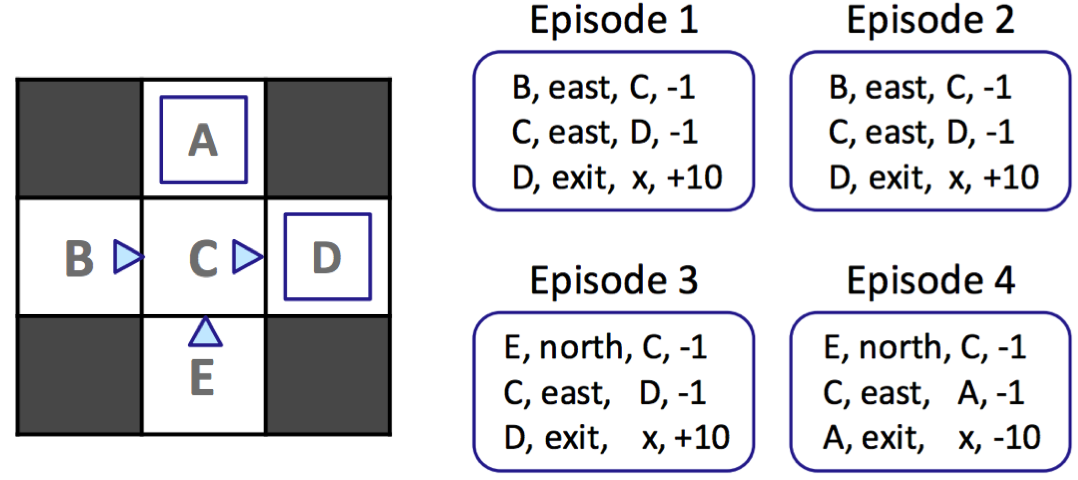
\includegraphics[width=12cm]{img/rl-example-1-full}
	\end{center}
Walking through the first episode, we can see that from state $D$ to termination we acquired a total reward of $10$, from state $C$ we acquired a total reward of $(-1) + 10 = 9$, and from state $B$ we acquired a total reward of $(-1) + (-1) + 10 = 8$. Completing this process yields the total reward across episodes for each state and the resulting estimated values as follows:
\begin{center}
\begin{tabular}{ |c|c|c|c| } 
 \hline
 \textbf{s} & \textbf{Total Reward} & \textbf{Times Visited} & \textbf{$V^{\pi}(s)$} \\ 
 \hline
 $A$ & $-10$ & $1$ & $-10$ \\
 \hline
 $B$ & $16$ & $2$ & $8$ \\ 
 \hline
 $C$ & $16$ & $4$ & $4$ \\
 \hline
 $D$ & $30$ & $3$ & $10$ \\ 
 \hline
 $E$ & $-4$ & $2$ & $-2$ \\ 
 \hline
\end{tabular}
\end{center}
Though direct evaluation eventually learns state values for each state, it's often unnecessarily slow to converge because it wastes information about transitions between states.
	\begin{center}
		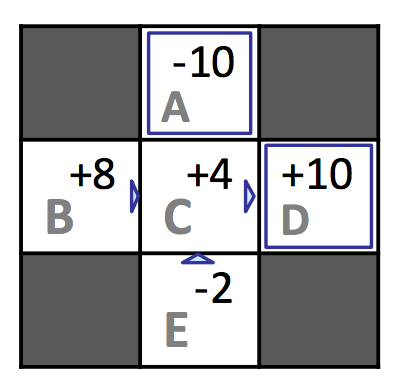
\includegraphics[width=5cm]{img/rl-example-1-annotated}
	\end{center}
In our example for, we computed $V^{\pi}(E) = -2$ and $V^{\pi}(B) = 8$, though both states only have $C$ as a successor state and incur the same reward of $-1$ when transitioning to $C$. According to the Bellman equation, this means that both $B$ and $E$ should have the same value under $\pi$. However, of the $4$ times our agent was in state $C$, it transitioned to $D$ and reaped a reward of $10$ three times and transitioned to $A$ and reaped a reward of $-10$ once. It was purely by chance that the single time it received the $-10$ reward it started in state $E$ rather than $B$, but this severely skewed the estimated value for $E$. With enough episodes, the values for $B$ and $E$ will converge to their true values, but cases like this may cause the process to take longer than we'd like. This issue can be mitigated by choosing to use our second passive reinforcement learning algorithm, temporal difference learning.

\subsection*{Temporal Difference Learning}
Temporal difference learning (TD learning) uses the idea of \textit{learning from every experience}, rather than simply keeping track of total rewards and number of times states are visited and learning at the end as direct evaluation does. In policy evaluation, we used the system of equations generated by our fixed policy and the Bellman equation to determine the values of states under that policy (or used iterative updates like with value iteration).
$$V^{\pi}(s) = \sum_{s'}T(s, \pi(s), s')[R(s, \pi(s), s') + \gamma V^{\pi}(s')]$$
Each of these equations equates the value of one state to the weighted average over the discounted values of that state's successors plus the rewards reaped in transitioning to them. TD learning tries to answer the question of how to compute this weighted average without the weights, cleverly doing so with an \textbf{exponential moving average}, explained below. We begin by initializing $\forall s, \:\: V^{\pi}(s) = 0$. At each timestep, an agent takes an action $a$ from a state $s$, transitions to a state $s'$, and receives a reward $R(s, \pi(s), s')$. We can obtain a \textbf{sample value} by summing the received reward with the discounted current value of $s'$ under $\pi$:
$$sample = R(s, \pi(s), s') + \gamma V^{\pi}(s')$$
This sample is a new estimate for $V^{\pi}(s)$. The next step is to incorporate this sampled estimate into our existing model for $V^{\pi}(s)$ with the exponential moving average by adhering to the following update rule:
$$V^{\pi}(s) \leftarrow (1-\alpha)V^{\pi}(s) + \alpha \cdot sample$$
Above, $\alpha$ is a parameter constrained by $0 \leq \alpha \leq 1$ known as the \textbf{learning rate} that specifies the weight we want to assign our existing model for $V^{\pi}(s)$ and the weight we want to assign our new sampled estimate. It's typical to start out with learning rate of $\alpha = 1$, accordingly assigning $V^{\pi}(s)$ to whatever the first $sample$ happens to be, and slowly shrinking it towards $0$, at which point all subsequent samples will be zeroed out and stop affecting our model of $V^{\pi}(s)$. 

Let's stop an analyze the update rule for a minute. Annotating the state of our model at different points in time by defining $V^{\pi}_k(s)$ and $sample_k$ as the estimated value of state $s$ after the $k^{th}$ update and the $k^{th}$ sample respectively, we can reexpress our update rule:
$$V^{\pi}_{k}(s) \leftarrow (1-\alpha)V^{\pi}_{k-1}(s) + \alpha \cdot sample)k$$
This recursive definition for $V^{\pi}_k(s)$ happens to be very interesting to expand:
\begin{eqnarray*}
	V^{\pi}_{k}(s) &\leftarrow& (1-\alpha)V^{\pi}_{k-1}(s) + \alpha \cdot sample_k \\
	V^{\pi}_{k}(s) &\leftarrow& (1-\alpha)[(1-\alpha)V^{\pi}_{k-2}(s) + \alpha \cdot sample_{k-1}] + \alpha \cdot sample_k \\
	V^{\pi}_{k}(s) &\leftarrow& (1-\alpha)^2V^{\pi}_{k-2}(s) + (1-\alpha) \cdot \alpha \cdot sample_{k-1} + \alpha \cdot sample_k \\
	\vdots \\
	V^{\pi}_{k}(s) &\leftarrow& (1-\alpha)^kV^{\pi}_0(s) + \alpha \cdot [(1-\alpha)^{k-1} \cdot sample_1 + \hdots + (1-\alpha) \cdot sample_{k-1} + sample_k] \\
	V^{\pi}_{k}(s) &\leftarrow& \alpha \cdot [(1-\alpha)^{k-1} \cdot sample_1 + \hdots + (1-\alpha) \cdot sample_{k-1} + sample_k]
\end{eqnarray*}
Because $0 \leq (1 - \alpha) \leq 1$, as we raise the quantity $(1 - \alpha)$ to increasingly larger powers, it grows closer and closer to $0$. By the update rule expansion we derived, this means that older samples are given exponentially less weight, exactly what we want since these older samples are computed using older (and hence worse) versions of our model for $V^{\pi}(s)$! This is the beauty of temporal difference learning - with a single straightfoward update rule, we're able to
\begin{itemize}
	\item learn at every timestep, hence using information about state transitions as we get them since we're using iteratively updating versions of $V^{\pi}(s')$ in our samples rather than waiting until the end to perform any computation. 
	\item give exponentially less weight to older, less accurate samples.
	\item converge to learning true state values much faster with fewer episodes than direct evaluation.
\end{itemize}
As a brief aside to our analysis, it's fairly common to see the TD learning update rule written as
$$V^{\pi}(s) \leftarrow V^{\pi}(s) + \alpha \cdot (sample - V^{\pi}(s))$$
which is identical, with just some basic algebraic manipulation applied. However, this second notation for the update rule gives us a slightly different but equally valuable interpration of the update: it's computing the difference between the sampled estimated and the current model of $V^{\pi}(s)$, and shifting the model in the direction of the estimate, with the magnitude of the shift being proportional to the magnitude of the difference.
\begin{center}
	<TODO: EXAMPLE FOR TD LEARNING>
\end{center}

\subsection*{Q-Learning}
Both direct evaluation and TD learning will eventually learn the true value of all states under the policy they follow. However, they both have a major inherent issue - we want to find an optimal \textit{policy} for our agent, which requires knowledge of the q-values of states. To compute q-values from values the values we have, this requires a transition function and reward function, as dictated by the Bellman equation.
$$Q^*(s, a) = \max_a \sum_{s'} T(s, a, s')[R(s, a, s') + \gamma V^*(s')]$$
As a result, TD learning or direct evaluation typically are used in tandem with some model-based learning to acquire estimates of $T$ and $R$ in order to effectively update the policy followed by the learning agent. This became avoidable by a revolutionary new idea known as \textbf{Q-learning}, which proposed learning the q-values of states directly, bypassing the need to ever know any values, transition functions, or reward functions. As a result, Q-learning is entirely model-free. Q-learning uses the following update rule to perform q-value iteration:
$$Q_{k+1}(s, a) \leftarrow \sum_{s'}T(s, a, s')[R(s, a, s') + \gamma \max_{a'} Q_k(s', a')]$$
Note that this update is only a slight modification over the update rule for value iteration. Indeed, the only real difference is that the position of the $\max$ operator over actions has been changed since we select an action before transitioning when we're in a state, but we transition before selecting a new action when we're in a q-state. 

With this new update rule under our belt, Q-learning is derived essentially the same way as TD learning, by acquiring \textbf{q-value samples}:
$$sample = R(s, a, s') + \max_{a'}Q(s', a')$$
and incoporating them into an exponential moving average.
$$Q(s, a) \leftarrow (1-\alpha)Q(s, a) + \alpha \cdot sample$$
As long as we spend enough time in exploration and decrease the learning rate $\alpha$ at an appropriate pace, Q-learning learns the optimal q-values for every q-state. This is what makes Q-learning so revolutionary - while TD learning and direct evaluation learn the values of states under a policy and can then determine whether the policy is optimal via other techniques, Q-learning can learn the optimal policy directly even by taking suboptimal or random actions. This is called \textbf{off-policy learning} (contrary to direct evaluation and TD learning, which are examples of \textbf{on-policy learning}).

\subsection*{Approximate Q-Learning}
Q-learning is an incredible learning technique that continues to sit at the center of developments in the field of reinforcement learning. Yet, it still has some room for improvement. As it stands, Q-learning just stores all q-values for states in tabular form, which is not particularly efficient given that most applications of reinforcement learning have several thousands or even millions of states. This means we can't visit all states during training and can't store all q-values even if we could for lack of memory.
\begin{center}
\begin{figure}[!h]
\minipage{.32\textwidth}
  \centering
  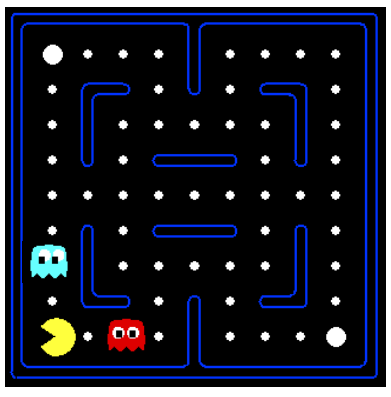
\includegraphics[width=.75\linewidth]{img/qlearn-pac-1}
  \caption{}
  \label{fig:sub1}
\endminipage\hfill
\minipage{.32\textwidth}
  \centering
  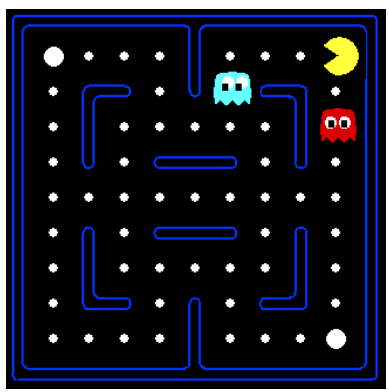
\includegraphics[width=.75\linewidth]{img/qlearn-pac-2}
  \caption{}
  \label{fig:sub2}
\endminipage\hfill
\minipage{.32\textwidth}
  \centering
  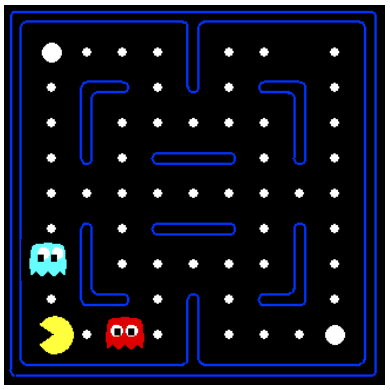
\includegraphics[width=.75\linewidth]{img/qlearn-pac-3}
  \caption{}
  \label{fig:sub3}
\endminipage
\label{fig:test}
\end{figure}
\end{center}
\vspace{-7mm}
 Above, if Pacman learned that Figure 1 is unfavorable after running vanilla Q-learning, it would still have no idea that Figure 2 or even Figure 3 are unfavorable as well. $\textbf{Approximate Q-learning}$ tries to account for this by learning about a few general situations and extrapolating to many similar situations. The key to generalizing learning experiences is the \textbf{feature-based representation} of states, which represents each state as a vector known as a \textbf{feature vector}. 
\begin{center}
	<TODO: ADD LEAST SQUARES PROOF OF APPROX QLEARNING>
\end{center}

\section*{Exploration and Exploitation}
We've now covered several different methods for an agent to learn an optimal policy, and harped on the fact that "sufficient exploration" is necessary for this without really elaborating on what's really meant by "sufficient". In the upcoming two sections, we'll discuss two methods for distributing time between exploration and exploitation: $\epsilon$-greedy policies and exploration functions.

\subsection*{{\LARGE$\varepsilon$}-Greedy Policies}
Agents following an \textbf{$\epsilon$-greedy policy} define some probability $0 \leq \epsilon \leq 1$, and act randomly and explore with probability $\epsilon$. Accordingly, they follow their current established policy and exploit with probability $(1 - \epsilon)$. This is a very simple policy to implement, yet can still be quite difficult to handle. If a large value for $\epsilon$ is selected, then even after learning the optimal policy, the agent will still behave mostly randomly. Similarly, selecting a small value for $\epsilon$ means the agent will explore infrequently, leading Q-learning (or any other selected learning algorithm) to learn the optimal policy very slowly. To get around this, $\epsilon$ must be manually tuned and lowered over time to see results.

\subsection*{Exploration Functions}
This issue of manually tuning $\epsilon$ is avoided by \textbf{exploration functions}, which use a modified q-value iteration update to give some preference to visiting less-visited states. The modified update is as follows:
$$Q(s, a) \leftarrow (1-\alpha)Q(s, a) + \alpha \cdot [R(s, a, s') + \max_{a'} f(s', a')]$$
where $f$ denotes the exploration function. There exists some degree of flexibility in designing an exploration function, but a common choice is to use 
$$f(s, a) = Q(s, a) + \frac{k}{N(s, a)}$$
with $k$ being some predetermined value, and $N(s, a)$ denoting the number of times q-state $(s, a)$ has been visited. Agents in a state $s$ always select the action that has the highest $f(s, a)$ from each state, and hence never have to make a probabilistic decision between exploration and exploitation. This decision is automatically encoded by the exploration function, since the term $\frac{k}{N(s, a)}$ can give enough of a "bonus" to some infrequently-taken action such that it is selected over actions with higher q-values. As time goes on and states are visited more frequently, this bonus decreases towards $0$ for each state and $f(s, a)$ regresses towards $Q(s, a)$, making exploitation more and more exclusive.

\section*{Summary}
It's very important to remember that reinforcement learning has an underlying MDP, and the goal of reinforcement learning is to solve this MDP by deriving an optimal policy. The difference between using reinforcement learning and using methods like value iteration and policy iteration is the lack of knowledge of the transition function $T$ and the reward function $R$ for the underlying MDP. As a result, agents must \textit{learn} the optimal policy through online trial-by-error rather than pure offline computation. There are many ways to do this:
	\begin{itemize}
		\item Model-based learning - Runs computation to estimate the values of the transition function $T$ and the reward function $R$ and uses MDP-solving methods like value or policy iteration with these estimates.
		\item Model-free learning - Avoids estimation of $T$ and $R$, instead using other methods to directly estimate the values or q-values of states.
			\begin{itemize}
			\item Direct evaluation - follows a policy $\pi$ and simply counts total rewards reaped from each state and the total number of times each state is visited. If enough samples are taken, this converges to the true values of states under $\pi$, albeit being slow and wasting information about the transitions between states.
			\item Temporal difference learning - follows a policy $\pi$ and uses an exponential moving average with sampled values until convergence to the true values of states under $\pi$. TD learning and direct evaluation are examples of on-policy learning, which learn the values for a specific policy before deciding whether that policy is suboptimal and needs to be updated.
			\item Q-Learning - learns the optimal policy directly through trial and error with q-value iteration updates. This an example of on-policy learning, which learns an optimal policy even when taking suboptimal actions.
			\item Approximate Q-Learning - does the same thing as Q-learning but uses a feature-based representation for states to generalize learning.
			\end{itemize}
	\end{itemize}
\end{document}